\documentclass[12pt,a4paper]{report}

\newenvironment{tightcenter}{%
  \setlength\topsep{0pt}
  \setlength\parskip{0pt}
  \begin{center}
}{%
  \end{center}
}

%%% User packages
\usepackage{wrapfig}
\usepackage{afterpage}
\usepackage{parskip} % Disable US-type paragraph
\usepackage[hyphens]{url}
\usepackage{titlesec}
\usepackage{xfrac}
\usepackage[usenames,dvipsnames,svgnames,table]{xcolor}
\usepackage{lastpage}
\usepackage{tocloft}
\usepackage{float}
\usepackage{fancybox, graphicx}
\usepackage[footnote,draft,english,silent,nomargin]{fixme}

%%% Tag specific
%\usepackage{tabularx} % Table
\usepackage{booktabs} % Nice tabelsMost critical path with backtracing
\usepackage{fancyhdr} % header & footer

%%% Layout related
\usepackage[left=2.5cm,right=2.5cm,top=2.5cm,bottom=2.5cm]{geometry} % Page margin

%%% Reference related
\usepackage{cleveref}
\usepackage[backend=bibtex]{biblatex}

%%% TOC
\setcounter{tocdepth}{1}

\bibliography{Kilder/kilder.bib}
%\PassOptionsToPackage{hyphens}{url}

%%% Font related
\usepackage{kmath,kerkis}
\usepackage{microtype}
\usepackage{mathptmx}
\usepackage[T1]{fontenc} 
\usepackage[utf8]{inputenc} %%\usepackage[utf8x]{inputenc}
\usepackage{amsfonts} % Math 
\usepackage[font=scriptsize]{caption} %small caption text

%%% Codeinput related
\usepackage[ruled]{algorithm2e}
\usepackage{listings} % Så man kan indsætte pæn kode, spørg Anders for hjælp
\usepackage{color}
\lstdefinelanguage{CSharp}
{
sensitive=false,
morekeywords=[1]{
abstract, as, base, break, case,
catch, checked, class, const, continue,
default, delegate, do, else, enum,
event, explicit, extern, false,
finally, fixed, for, foreach, goto, if,
implicit, in, interface, internal, is,
lock, namespace, new, null, operator,
out, override, params, private, foreach
protected, Task, Tasks, List, public, readonly, ref,
return, sealed, sizeof, var, stackalloc,
static, struct, switch, this, throw,
true, try, typeof, unchecked, TimeSpan, unsafe,
using, virtual, volatile, while, bool,
byte, char, decimal, double, float,
int, lock, object, sbyte, short, string,
uint, ulong, ushort, void, get, set},
morecomment=[l]{//},
morecomment=[s]{/*}{*/},
morecomment=[l][keywordstyle4]{\#},
morestring=[b]",
morestring=[b]',
}
\lstset{
backgroundcolor=\color[rgb]{0.95, 0.95, 0.95},
tabsize=2,
rulecolor=,
basicstyle=\scriptsize,
upquote=true,
aboveskip={1.5\baselineskip},
columns=fixed,
showstringspaces=false,
extendedchars=true,
breaklines=true,
frame=single,
showtabs=false,
showspaces=false,
showstringspaces=false,
identifierstyle=\ttfamily,
keywordstyle=\color[rgb]{1.0,0,0},
keywordstyle=[1]\color[rgb]{0,0,0.75},
keywordstyle=[2]\color[rgb]{0.5,0.0,0.0},
keywordstyle=[3]\color[rgb]{0.127,0.427,0.514},
keywordstyle=[4]\color[rgb]{0.4,0.4,0.4},
commentstyle=\color[rgb]{0.133,0.545,0.133},
stringstyle=\color[rgb]{0.639,0.082,0.082},
} % Dokument der tilader at bruge C# farvestil i kode indsættelse
\lstset{language=[Sharp]C} 
\lstdefinestyle{csharp2}{language=[Sharp]C, frame=lr, rulecolor=\color{blue!80!black}}

\makeatletter
\renewcommand\part{%
    \if@openright
        \cleardoublepage
    \else
        \clearpage
    \fi
    \thispagestyle{empty}%
    \if@twocolumn
        \onecolumn
        \@tempswatrue
    \else
        \@tempswafalse
    \fi
    \null\vfil
    \secdef\@part\@spart}
\makeatother

\AtBeginDocument{\addtocontents{toc}{\protect\thispagestyle{empty}}} 

\titleformat{\chapter}{\normalfont\huge\bfseries}{ \thechapter.}{20pt}{\huge}
\setcounter{section}{0}
\pagestyle{fancy}
\fancypagestyle{arabic}
{
    \fancyhf{}
    \setlength{\headheight}{15pt}
}



%\titleformat{\chapter}[display]   
%{\normalfont\huge\bfseries}{\chaptertitlename\ \thechapter}{20pt}{\Huge}   
\titlespacing*{\chapter}{-10pt}{-20pt}{10pt}

\renewcommand{\chaptermark}[1]{ \markboth{#1}{} }
\fancypagestyle{chp}{
  \fancyhf{}
    \lhead{\MakeUppercase{\leftmark}}
  \rhead{\rightmark}%\colorbox{black}{\color{white}{\rightmark}}}
  \cfoot{\thepage\ of \pageref{LastPage}}
}
\fancypagestyle{plain}{
    %\fancyhf{}
  \cfoot{\thepage\ of \pageref{LastPage}}
}

\newcommand*{\blankpage}{%
\vspace*{\fill}
\centering \textit{This page intentionally left (almost) blank.}
\vspace{\fill}}

\pagestyle{fancy}

\title{
    \vspace*{-3cm}
    \fontsize{50}{48} \textbf{Titel TBA}\\
    \fontsize{20}{48}\emph{A software analysis and -implementation}
}
\author{
    \noindent\makebox[\textwidth]{%
    
\includegraphics[width=1.2\textwidth]{Grafik/ForsideUmodificeret.png}\hspace*{0.5cm}}\\
    \emph{Mathias Vestergaard Rasmussen}\\
    \emph{Christoffer Carlé Christensen}\\
    \emph{Kasper Østergaard Helsted}\\
    \emph{Anders Lykke Matthiassen}\\
    \emph{Christian Stephansen}\\
    \emph{Gideon Blegmand}
}

\date{19 - 12 - 2014}


\definecolor{codecomment}{HTML}{383838}

\lstset{language=C,
    basicstyle=\ttfamily\scriptsize,
    keywordstyle=\color{Blue}\ttfamily,
    otherkeywords={WIDTH},
    keywords=[2]{__shared__},
    keywordstyle=[2]\color{orange}\ttfamily,
    stringstyle=\color{red}\ttfamily,
    commentstyle=\color{codecomment}\ttfamily,
    breaklines=true,
    numbers=left,
}

\usepackage[bookmarks]{hyperref}
\hypersetup{pdftex, hidelinks=true}
\usepackage{hypcap}
\DeclareUnicodeCharacter{00A0}{~}

\begin{document}
    \addtocontents{toc}{\protect\thispagestyle{empty}}
    \maketitle
    \afterpage{\blankpage}
        \thispagestyle{empty}
    %\pagenumbering{gobble}
    \clearpage
    %Titlepage 
    \thispagestyle{empty}
\begin{titlepage}
    \setlength{\textwidth}{15cm}
    \noindent
    \begin{nopagebreak}
        {\samepage 
            \begin{tabular}{lr}
                \parbox{0.5\textwidth}{\raisebox{11mm}
                    {
\includegraphics[height=2.2cm]{Grafik/aauLogoDa2}}
                } &
                \parbox{0.5\textwidth}{
                    \small
                    \begin{tabular}{l}
                        {\sf\small \textbf{Department of Computer Science }}\\
                        {\sf\small CASSIOPEIA} \\
                        {\sf\small Selma Lagerløfs Vej 300} \\
                        {\sf\small DK-9220 Aalborg Ø.} \\
                    \end{tabular}
                }
            \end{tabular}
            
            \noindent
            \begin{tabular}{cc}
                \parbox{7cm}{
                    \begin{description}
            
                        \item {\bf Title:} 
            
                            \textbf{Meal Planner}\\
                        \item {\bf Project Period:}\\
                            Autumn Semester 2014\\
                            \hspace{4cm}
                        \item {\bf Project Group:}\\
                            SW3-ds301e14\\
                            \hspace{4cm}
                        \item {\bf Participants:}\\
                            Mathias Vestergaard Rasmussen\\
                            Christoffer Carlé Christensen\\
                            Kasper Østergaard Helsted\\
                            Anders Lykke Matthiassen\\
                            Christian Stephansen\\
                            Gideon Blegmand\\
                            \hspace{2cm}
                        \item {\bf Supervisor:}\\
                            Rudra Pratap Deb Nath\\

                        \item {\bf Copies:}\\ 9\\
                        \item {\bf Page Numbers:}\\ 117\\
                        \item {\bf Appendix:}\\ Page 92-117\\
                        \item {\bf Date of Completion:}\\ 19-12-2014\\
                    \end{description}
                    \vfill
                } &
                \parbox{7cm}{
                    \vspace{.15cm}
                    \hfill 
                    \begin{tabular}{l}
                        {\bf Abstract:}\bigskip \\
                        \fbox{
                            \parbox{6.5cm}{\smallskip
                                {\vfill{\small %\section* {Synopsis}

                                \smallskip}}
                            }
                        }
                    \end{tabular}
                }
            \end{tabular}
        }\\
        \\
        \noindent{\footnotesize\emph{The contents of this report is freely accessible, but publication (with referencing) may only happen under agreement with the authors.}}
    \end{nopagebreak}
\end{titlepage}

    \afterpage{\blankpage}
        \thispagestyle{empty}
    %\pagenumbering{gobble}
    \clearpage
    %\pagenumbering{roman}
    \chapter*{Preface} \label{PrefaceLabel}

This report is a result of the hard work of Anders Lykke Matthiassen, Christian Stephansen, Christoffer Carlé Christensen, Gideon Blegmand, Kasper Østergaard Helsted, and Mathias Vestergaard Rasmussen.

The intellectual property rights of this report and all of its contents belong to the members of the project. All material gathered from third party resources will be referred to according to the IEEE standard.

The source code for the software solution of the project, is open source, under the Beerware license. The code is freely available at https://github.com/Helstedxd/FoodPlanner-Project.

The colours for this program, were chosen by using an online tool called Paletton \cite{paletton}, which suggests a colour theme based on the colours the user choose. The figures used in the report, have been created using Visio and Inkscape, unless stated otherwise.

The authors would like to thank participants of the Usability test for their time and constructive critique, as well as the informants for the interviews and user stories, for their cooperation. The report makers would also like to thank Rudra Pratap Deb Nath for his help and constructive criticism throughout the project process.

        \thispagestyle{empty}
    %\renewcommand*\contentsname{Indholdsfortegnelse}
    \newpage
        {\pagestyle{empty}
    \tableofcontents
    \cleardoublepage}
    \pagenumbering{arabic}
    \clearpage
    \setcounter{page}{1}
    \pagestyle{plain}
    
    \part{Problem Analysis}
    	\section{Foodplan study}
\textit{Stop Spild Af Mad}\cite{madSpild_RapportAdfaerd} has conducted a study where eight informants had had to create and follow a weekly food-schedule.
Each participants had to create a foodplan and they could freely choose the different recipes with inspiration from cookbooks or the internet.

\subsection*{Planning}
The informants had some trouble with pulling them self together and getting started creating the foodplan, but they were happy to have it, once it was done. It could be beneficial for the person that were in charge of grocery-shopping, to be the one making the schedule, since the involvement of other members from the family could increase the time of making it.

\subsection*{Modules}
It was almost impossible for the informants to follow the schedule for a whole week, without having to reorganize or modify it. Most of the informants made small modules, that could be moved around depending on the family's situation. It was optimal with modules spanning two-three days. Varied meals was preferred, and not simply reheated meals.

\subsection*{grocery-shopping}
Seven out of the eight participants was shopping groceries almost every day. This was not seen as a nuisance, but after having planned grocery-shopping for a whole week, they experienced a big relief in their everyday life. This was expressed in terms of more personal freedom as a consequence of saving time and money. Planning ahead also decreased buying on impulse.
\fxnote{textbf might be a bad choice.. CHS tried using emphasize on Less gro... and subsubsec on Modules (subsubsec throws a warning because we have no subsec beforehand .. please evaluate, on which type we should use.}

\subsection{Reflection} \fxnote{This is some sort of conclusion/reflection for this section, but might need to be moved.}
The participant had trouble getting started creating a new food plan for the week. They also wanted a more realistic food-schedule instead of having to create it from cookbooks. Realistic in the sense that the plan should fit into their context. A solution to this problem might be solved by automating a lot of the tasks involved with having to come up with the different recipes and do the grocery shopping.
By having an application come up with suggested meals based on different aspects such as the:
\begin{itemize}
\item Food you already have
\item Food you like
\item Price
\item Stock of stores nearby
\end{itemize}
People could quickly create the schedule or maybe even have the application create it for them.
\section{FDB Report}
The following section examines a report published in 2011 by FDB called "Forbrugerne: Vi smider ikke mad ud"\cite{madSpild_FDB}.
\subsection{Method used in the report}
The report is an anthropological study of how food waste occurs and how it is experienced by the consumers. The study is based on qualitative data collected from six different households. These households are all different from one another e.g. they live in different geographical locations. Data is gathered from the participants by using observations e.g. watching participants shop or prepare food, semi-structured interviews and probing kits. The data is then used to examine the activity patterns and motivation of the participants.

\subsection{FDB report: What is food waste and how does it occur.}
The report discusses why food waste occurs and how the participants perceive it. There are some subjects that are interesting when learning about food waste. 

\subsubsection{What is food waste}
When the participants was asked how much food they threw out, they typically answered that they threw out as little as possible. There is a clear distinction between waste and non-waste being thrown out. It is acceptable to throw waste out, but not to do the same with non-waste. The waste and non-waste categories varies depending on cooked food products and uncooked food products. Cooked food is considered waste when larger parts, or leftovers of a meal that has not been served on a plate is thrown out. So when the food has been served on a plate it is acceptable to throw it out. Uncooked food is considered waste when the packaging is unopened. It is not considered waste when the uncooked fat or other food parts that are considered non-edible is thrown out.

\subsubsection{Cause of food waste} 
The reasons as to why food is thrown out varies depending on cooked and uncooked products. Uncooked products is thrown out because they are bought in so large quantities that the consumers were not able to eat it prior to expiry. Products that are considered non-edible such as cartilage or bad vegetables are also thrown out. Cooked food products are also likely to be thrown out. Cooked food products are thrown out because the participants prepared more than they could eat in one meal. If the participants estimated that there were enough leftovers to save them for later they would. But often the leftovers was stored in the fridge for 4 days only to be thrown out.

\subsubsection{Food waste barriers}
The participants might have the will to reduce food waste but there are some barriers that can impact the participants will in a negative way. The status \fxnote{status/value formulation} of the meal ingredients can be a barrier. Dinner is often based around the chosen kind of meat because it has more value. This means that all other ingredients on a plate only is supplementary. It is easier to throw away the supplements than the meat because of its status. Therefore supplements represents a larger part of the food waste in the homes. Making a large delicious and fresh meal is also a way to show appreciation towards guests or household members. This can also act as a barrier because it requires the food to be fresh and in large amounts. Another barrier is quantity discounts. It contradicts with the participants reasoning when they have to decide between buying what is the right economical, or what is right according to food waste. In the situation people often think of the economical aspects, and not on what they will do with the extra food. The participants also expressed a lack of overview of what products they had at home when they were out shopping. Sometimes they bought something that they already had, because they was not sure if they had it at home. This results in an overstocking of a product that is most likely to be thrown out. Another barrier was planning versus impulse and desire. Participants that shopped regularly, said that they sometimes changed their minds on what they wanted for dinner or that they wanted variation in their dinners. This spontaneity and need for variation could result in products being bought for one night and the leftovers being stored and in the end being thrown out. Participants that shopped frequently said that they wanted variation and therefore did not plan dinners for a whole week. This could result in a lack of overview and in the end more food waste. The expiration date can also affect the participants willingness to buy a product. The tolerance of when a product is not edible varies between participants, and when the product can give a smell or a visual sign of decay. The expiration date had less importance. The last barrier that is discussed is what is acceptable as food waste. Some of the barriers that has been mentioned is accepted in some degree by the participants. One of the participants talks about the acceptance of food waste when it comes from a child's plate. The participants says that it is to hard assess how much the child will eat and that it leads to food waste but it is a waste the participant will accept.
\section{How to avoid food waste}

According to The Danish Ministry of the Environment, one of the initiatives you can take against food waste, is to make recipes which incorporate the leftovers, or what is left in the refrigerator. By doing this food that might otherwise go bad, will be used instead of being thrown away. http://mindremadspild.dk/files/mindremadspild_idekatalog_150611.pdf

Another Initiative that can be taken according to The Danish Ministry of the Environment, is to sell quantity discount, with the option to recieve some of the groceries later. An example would be if 1 cucumber is sold for 10 DKK, while 2 is sold for 15, some people would choose to buy 2 cucumbers because of the quantity discount, even if they just needed 1 at the moment. With a "recieve later" option, you would be able to buy 2 cucumbers, but only recieve 1 at the moment. Then you would be able to come back to the store later to get the other cucumber when you needed it. An initiative like this have already been made by the English supermarket chain Tesco. The initiative is called "Buy One Get One Free Later", and is an initiative for fresh groceries like fruit and vegetables.

To give the consumer better information about when food is going bad is also an initiative that The Danish Ministry of Environment is recommending. By informing consumers of what "Best before", "Last day of sale" and so on means, would get the consumer to use the food more properly. Also by getting the consumer to rely more on smell, taste and looks, rather than just the date of production on the groceries, would lead to lesser food waste.

The Danish Ministry of the Environment, also reccomend getting discounts even thoug you don't buy in quantity. Being able to share an offer with another person would let the supermarkets get volumes bought, and the consumer would be able to only aquire the amount neccessairy.

Only using the gorecries neccessairy is also a way to achieve lesser food waste. Following Recipes will help with this if the recipes is specific. If for example the repicipe is for 4 persons, and 4 persons will be eating, if the recipe is correct food will not be wasted, and even if there are leftovers after the meal, using these as lunch for the next day, or eating the leftovers the day after, will achieve a lesser waste of food. http://www.brugmerespildmindre.dk/mindre-madspild


\section{Food waste}
Every year danish households throws away nearly 237.000 tons of food, that could have been eaten by people. This is estimated to be nearly 16 mio DKK. About 20 \% of a danish households foodbudget is wasted by throwing away food that could have been eaten, this means that if there was no food waste at all, 1 million people could be fed, this is nearly 1/5 of the danish people.

The people who throws away most food, are the people living alone. The average person living alone throws away 98.8 kg of food per year, where as a household with 5 people throws away 46.8 kg of food per person per year. It is mostly dairy products, vegetables and bread that gets thrown away, though in december a lot of meat is also thrown away, due to the fact that it is Christmas, where people eat more food.

Since 2007 the danish people have been purchasing 10 \% less food, a lot of this food used to end up in the trashcan as food waste. 54 \% of the danish people rarely or never uses the food from the night before for later eating, and 69 \% does not use leftovers for lunch the day after. Elderly people are better at using leftovers than younger people. \fxnote{references to bibliography, and/or maybe some graphs to show the numbers?}

20 \% of danish people does not make a grocery shopping list before going grocery shopping. 52 \% of people does not make a meal plan, 31 \% does sometimes and 17 \% does it often.

81 \% of danish people would use leftovers to avoid food waste, 50 percent would make a mealplan and make a grocery shopping list. 59 \% of the consumers believe that the danish food waste is their own fault.

\input{Analysis/StateOfTheArt.tex}

\chapter{PACT Analysis}
In this chapter, a pact analysis will be conducted in order to acquire a clearer view of how the main audience for the solution will behave. The information will be needed in order to find the requirements.
\section{People}
Everyone needs food, and many also have to buy and make it themselves. There are many ways to prepare a meal, and people have different preferences of what they eat and why. In this analysis the focus will be on the social, physical and psychological differences between people and on a description of their different motives and preferences. This description will be used to get an idea of who could benefit from a system, that would help them organize grocery shopping and preparing meals more efficiently.

\subsection{Physical differences}

People have different physical abilities. Some people have bad vision, some have bad hearing, and so on with a lot of different physical conditions, and taking this into considoration is an important aspect of a PACT analysis.

Looking at the ergonomically aspects of the application, is not necerrairy, since the ergonomics are decided by the company who creates the device that the application run on. Therefore ergonomics are not something that can be affected by the application.

\subsection{Psychological differences}

People vary in the way that they function psycologically. But some of the common traits to look at when designing software are:

\begin{itemize}
    \item The meaning of buttons
    \item Not too hard to remember instructions
\end{itemize}

The meaning of buttons is very important because depending on where the software will be released, buttons mean different things. Since the food planner application is going to be released in Denmark, it is therefore important that the danish people will percieve the buttons correctly.

It is also important that no instructions or commands are too long, because it will be hard to remember for some people, and when making a product you must take the weakest user into consideration when looking who to make the product for.

\subsection{Social differences}

People have different requirements of a product, and it is therefore important for the developer to make sure everyone can get, from the prodcut, what they want. Therefore some groups of peope with social differences will now be mentioned.

\subsubsection{People living after a special diet, or having specific wishes for food plans}
People that are on a specific diet needs to buy food based on the diet, and sometimes prepare it in a specific way.
Some examples of these people could be:
\begin{itemize}
\item Sports performers(Bodybuilders)
\item Vegans/vegetarians
\item Organically minded
\end{itemize}

\subsubsection{People who want to save time when making and planning cooking and doing the groceries} 
If people do not plan on what they are going to eat throughout the week, they often have to buy groceries everyday, and maybe the food they are preparing takes a longer time to cook than they expected. In this case an organized foodplan based on how long time it takes to prepare a meal and what groceries you have, could help save time in the everyday life. People who can benefit from saving time because of tight schedules can be:
\begin{itemize}
\item Students
\item Parents
\item Families
\end{itemize}\fxnote{Hvordan er vi kommet frem at disse mennesker hører til gruppen af dem som "want to save time when making and planning cooking and doing the groceries"}

\subsubsection{People who wants to be social while eating}
When people wants to get together and eat for different occasions, it could be beneficial if they plan the meal based on the preferences of the people involved.
These groups of people could be:
\begin{itemize}
\item Social eaters, people who only get together to eat a meal together
\item Students
\item Parents
\item People with a tight or small budget
\item Students
\item Parents
\end{itemize}\fxnote{Hvordan er vi kommet frem at disse mennesker hører til gruppen af dem som "wants to be social while eating" ??}

Some people might only want to eat with people of the same interests and food habits. These people includes:

\begin{itemize}
\item Vegans/vegetarians
\item Organically minded
\item Social eaters
\end{itemize}

\subsubsection{Comparison}
It is common for all the described people that they could save time and/or money by planning their grocery-shopping and meals. A system would have to be fast and easy to use, so that the time spent planning does not exceed the time it would normally take. The system should automate tasks for the user, for example by recommending recipes and keeping track of what food they already have at home. It must be very easy for the user to input the groceries, and not become a burden, preferably this should be fully automated, for example by adding groceries from a shopping list that a user used when shopping, or semi-automated by allowing the use to scan the product barcode.\fxnote{Nogle af de krav der bliver nævnt her kommer ud af den blå luft."The system should automate tasks for the user..." Hvad kommer det krav af?}

\fxnote{incorporate more family stuff}
\section{Activities}
To see in which context the program will be used, we first look at the activities associated with using the program. The activities have been split into two categories, what happens \textit{inside} and \textit{outside} of the home.

In the home:
\begin{itemize}
\item The program will be used to manage the food supply, by;
	\begin{itemize}
		\item Viewing a list of the stored groceries
		\item Updating the list, by adding or removing groceries that could have been used, or groceries that have gone bad
		\item "Flushing" the stored groceries. This should be done when the program is initiated for the first time or after a long period of inactivity
		\item Create a shopping list of the groceries needed for the planned meals
		\item Search for recipes
		\item Add new or modified recipes
	\end{itemize}
	Furthermore it should be in the home that preferences are set, which could be groceries you want to ignore, because;
	\begin{itemize}
		\item You do not like them
		\item You are allergic
		\item The grocery is not associated with a certain diet
	\end{itemize}
	Certain recipes will require the use of certain kitchen tools, therefore you would want to;
	\begin{itemize}
		\item View what tools are needed
		\item Be able to check if you have the kitchen tools
		\item Associate kitchen tools with a specific recipe
	\end{itemize}
	\item While cooking the meal, you would want to follow a recipe while cooking, which mean you might have to interact with the program during the cooking
\end{itemize}

Outside the home:
\begin{itemize}
\item While shopping for groceries, it is necessary to keep track of the shopping list, to see what should be bought.
\item If a new recipe is wanted on the fly, the shopping list must be updated
\end{itemize}

Frequent activities such as looking for a recipe should be easy to do, but some activities such as flushing the stored groceries should be easy to learn. This could be done by having a walkthrough when a user tries to do this particular activity. The program should also have easy navigation options to allow for mistakes to happen, such as going into undesired program pages, and still be able to get back on track. If the user is interrupted and have to pause their usage of the program, the user should be able to continue later from the same point. This is relevant if they are making a grocery list or a new recipe. These documents should have a save and edit function in order for the user to pick up on their work later.

The response time could become a point of frustration for the user if they want to lookup an online recipe and the response time is more than five seconds. As the recipes are available online there is a risk of high latency between a user's device and the server containing the recipes. A workaround for this could be to have a local version of the recipe database, and only have the device to synchronise the two databases once in a while.

The user is able to add or edit recipes and groceries to lists, and will therefore need an method of inputting alphabetic data into the program. Since the solution is minded to be on a handhold or mobile platform, a keyboard is not optimal as it will be frustrating to carry around. A small integrated keyboard, like the one a BlackBerry has\cite{blakBerry}, would not work either as it will get dirty when used in the kitchen. For example if the user is baking and want to type on the keyboard, flour could get in between the buttons, which would be difficult to clean. A touch display can simulate a keyboard and easily be cleaned with a towel and, and is therefore the best option for this solution. Voice recognition could also be a possibility, but outside noise will be too big of a nuisance. A lot of noise could interfere with the program when the user is in a mall or using kitchen tools such as a blender, or if they are boiling water.

    \part{Product Development}
		\chapter{Design}

\section{Personas}
This part will show three different personas.

\subsection{Henrik Jensen}
\begin{figure}[H]
	
\includegraphics[width=0.30\textwidth]{Grafik/FoodPlanner/PersonaHenrikJensen}
	\label{PersonaHenrikJensen}
\end{figure}
\begin{itemize}
	\item Age: 38
	\item Relational status: Married
	\item Children: 2, age 16 and 14
	\item Occupation: Working as an IT consultant.
	\item Preferences: Wanna spend less time on shopping but still cook delicious dinners.
\end{itemize}
-Henrik drives home after he has finished a meeting with a costumer. The meeting dragged on and Henrik Just want to get home and get a nice dinner.

-His wife is working as a nurse and has a late night shift this evening. It is therefore up to Henrik to cook Dinner for the whole family

-On his way home he stops by the local supermarket and on his way to the entrance he starts to plan what he will prepare for dinner.

-He finds some meat on sale which he decides to buy.

-When he gets home he finds the recipe he wanted and starts to cook.

-It annoys him slightly that he does not plan ahead and very variated. Bu he fells he ha no other choice because of his work schedule and his desire to reduce shopping time.

-After dinner he starts the washing machine and turns on tv to watch football. He is an football enthusiast and played it himself when he was younger. 

\subsection{Peter Nielsen}
\begin{figure}[H]
	
\includegraphics[width=0.15\textwidth]{Grafik/FoodPlanner/PersonaPeterNielsen}
	\label{PersonaHenrikJensen}
\end{figure}
\begin{itemize}
	\item Age: 23
	\item Relational status: Single
	\item Children: None
	\item Occupation: Student
	\item Preferences: Does not spend more time in the kitchen than needed.
\end{itemize}
-Peter has classes till late afternoon, so when he gets of school he rushes home, and does not care about dinner when he leaves school.

-Peter first plans what he is going to have for dinner when he get home. At this point he is usually just plans something that is fast to make.

-When he has to shop he goes for the nearest shop, and just buys what the recipe says, and does not look at what is on sale.

-When he gets home after buying the ingredients, he wait till he is hungry before starting making the food.

-He is slightly annoyed that he does not plan ahead but he blames that he has no things to help him seclude his plans.

-After dinner he starts he goes sit in front of the computer where he starts playing video games with his friends.

\subsection{Anne Madsen}
\begin{figure}[H]
	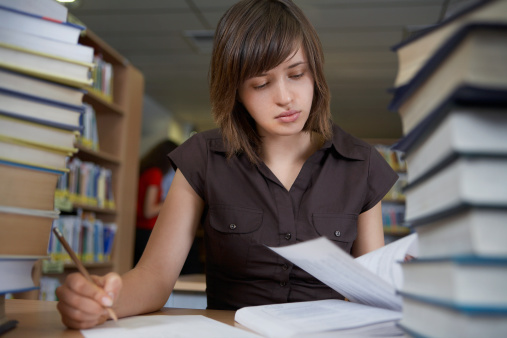
\includegraphics[width=0.25\textwidth]{Grafik/FoodPlanner/PersonaAnneMadsen}
	\label{PersonaHenrikJensen}
\end{figure}
\begin{itemize}
	\item Age: 18
	\item Relational status: Single
	\item Children: None
	\item Occupation: Student
	\item Preferences: Likes to spend time in the kitchen to prepare a good fresh meal with vegetables
\end{itemize}
-Anne has classes till late afternoon, after school Anne has a specific shopping list based on what she has to buy to make food for dinner.

-Anne does not know where to find the cheapest groceries which she finds slightly annoying, so she keeps shopping the same place as she has always done.

-When Anne is done shopping she decides that it is too dangerous to ride her bike with a bag of groceries hanging of her handlebar. So she decides to pull her bike home.

-When Anne finally gets home the trip from school to home has taken so long that it is time to make dinner.

-After dinner she cleans the plates, and gets ready to prepare her homework for the next day. 

\chapter{Problem Domain}
In this chapter the reality the user is going to see will be described. This reality is constructed of the areas which the system is going to administrate, monitor or control. Descriptions of classes, objects, structures and behaviours will be made throughout the chapter.


\section{Classes}\label{ClassesLabel}
In this section a list of classes will be presented. The classes described are those which have been chosen through a class candidate analysis.

\subsection{Physical}
\begin{itemize}
\item \textbf{Product:} This class is used to identify different ingredients for the recipes with information such as food type and expiration date. This class is essential for the program and will be used frequently.
\item \textbf{Recipe:} This class holds information about the ingredients and instructions on how to cook the meal.
\item \textbf{Scheduled Meal:} This class contains information about a recipe and when it is scheduled to be cooked.
\end{itemize}

\subsection{Persons}
\begin{itemize}
\item \textbf{User:} This class contains information about the preferences of a specific user, and will allow the solution to synchronise/share data with other users or devices.
\end{itemize}

\subsection{Places}
\begin{itemize}
\item \textbf{Shop:} This class holds information about the location of specific groceries and discounts.
\end{itemize}

\section{Events}
In this section a list of events will be presented. The events described are those which have been chosen through an event candidate analysis. The events and what trigger them are listed below.
\subsection{Consumption}
\begin{itemize}
\item \textbf{Product bought:} A shopping list have been completed. The items bought will be added to an inventory.
\item \textbf{Product removed:} A meal have been prepared and the product should be removed from the inventory, or have an subtraction from its original volume/quantity.
\item \textbf{Product expired:} When a product reaches its expiration date, it should be removed from the inventory and thrown out.
\end{itemize}

\subsection{Planning}
\begin{itemize}
    \item \textbf{Recipe scheduled:} When a recipe is scheduled for a date in the meal plan.
    \item \textbf{Recipe removed:} When the user removes a recipe which was scheduled for a date in the meal plan.
    \item \textbf{Shopping list item added:} When a recipe have been scheduled in the meal plan, missing ingredients from the inventory are added to the shopping list.
\end{itemize}

\subsection{Preferences/settings}
\begin{itemize}
\item \textbf{Preference changed:} When the user navigates to a settings menu to exclude products from the system, due to allergies, diets or preference.
\end{itemize}

\section{Event Table}
\Cref{tab:EventTable} shows an event table that have been constructed in order to get an overview of the relations between classes and events. The event table allows for a better judgement of which classes are relevant in the program. A plus (+) in the table indicates, that an event can occur zero or one time, whereas a star (*) indicates that an event can occur zero or more times.

\begin{table}[H]\centering
    \begin{tabular}{|r|c|c|c|c|}
        \hline
        ~                                      & Product & Recipe & User & Meal\\ \hline
        \textbf{Consumption}                   & ~       & ~      & ~    & ~   \\ 
		    Product added                          & +       & ~      & ~    & ~   \\ 
        Product removed                        & +       & ~      & ~    & ~   \\ 
        Product expired                        & *       & ~      & ~    & ~   \\ 
        Product unexpired                      & *       & ~      & ~    & ~   \\ 
        Product quantity changed               & *       & ~      & ~    & ~   \\ 
        Product expiration changed             & *       & ~      & ~    & ~   \\ 
        \textbf{Planning}                      & ~       & ~      & ~    & ~   \\ 
        Shopping list item added               & +       & ~      & ~    & ~   \\ 
        Meal added                             & ~       & +      & ~    & +   \\ 
        Meal removed                           & ~       & +      & ~    & +   \\ 
        Meal rescheduled                       & ~       & +      & ~    & +   \\ 
        Meal participants changed              & ~       & ~      & ~    & *   \\ 
        Meal Date changed                      & ~       & ~      & ~    & *   \\ 
        \textbf{Other}                         & ~       & ~      & ~    & ~   \\ 
        Preference changed                     & ~       & ~      & *    & ~   \\ 
		    Recipe found                           & ~       & *      & ~    & ~   \\ 
		\hline    
    \end{tabular}
    \caption{An event table for the program} 
    \label{tab:EventTable}
\end{table}
\section{Event Traces} \label{EventTraces}
This section will present a statemachine diagram for each class. Each statemachine diagram is the result of examining each class, with a focus on identifying the different states of the class' objects and the events, which effects the objects and changes their state. An event can happen without changing the state of the class e.g. on \cref{MealClass} the \textit{Change scale} event will not lead to a new state for the meal class object.  

Each class examination first shows a few of the event traces that were formulated for the specific class. The relationship between the classes and events are described in \cref{tab:EventTable}. The event traces will be used to model the statemachine diagram for the specific class. The event traces and statemachine diagrams are created to get a better understanding of the dynamic in the problem domain. It is possible to use the event definitions in \cref{EventsSection} for a better understanding of each event, if the event behaviour is not clear from the event name.   

\subsection{Food Class}
Some of the event traces used to understand the behaviour of this class are:
\begin{itemize}
	\item \textit{Added} -> \textit{Expired} -> \textit{Quantity changed} -> \textit{Removed}.
	\item \textit{Added} -> \textit{Quantity changed} -> \textit{Expired} -> \textit{Quantity changed} -> \textit{Unexpired} -> \textit{Removed}.
	\item \textit{Shopping list item added} -> \textit{Added} -> \textit{Expired} -> \textit{Removed}.
	\item \textit{Shopping list item added} -> \textit{Shopping list item removed}.
\end{itemize}

This class also has some event traces which are not legal e.g. 
\textit{Shopping list item added} -> \textit{Expired}.

\begin{figure}[tbhp]
	\centering
	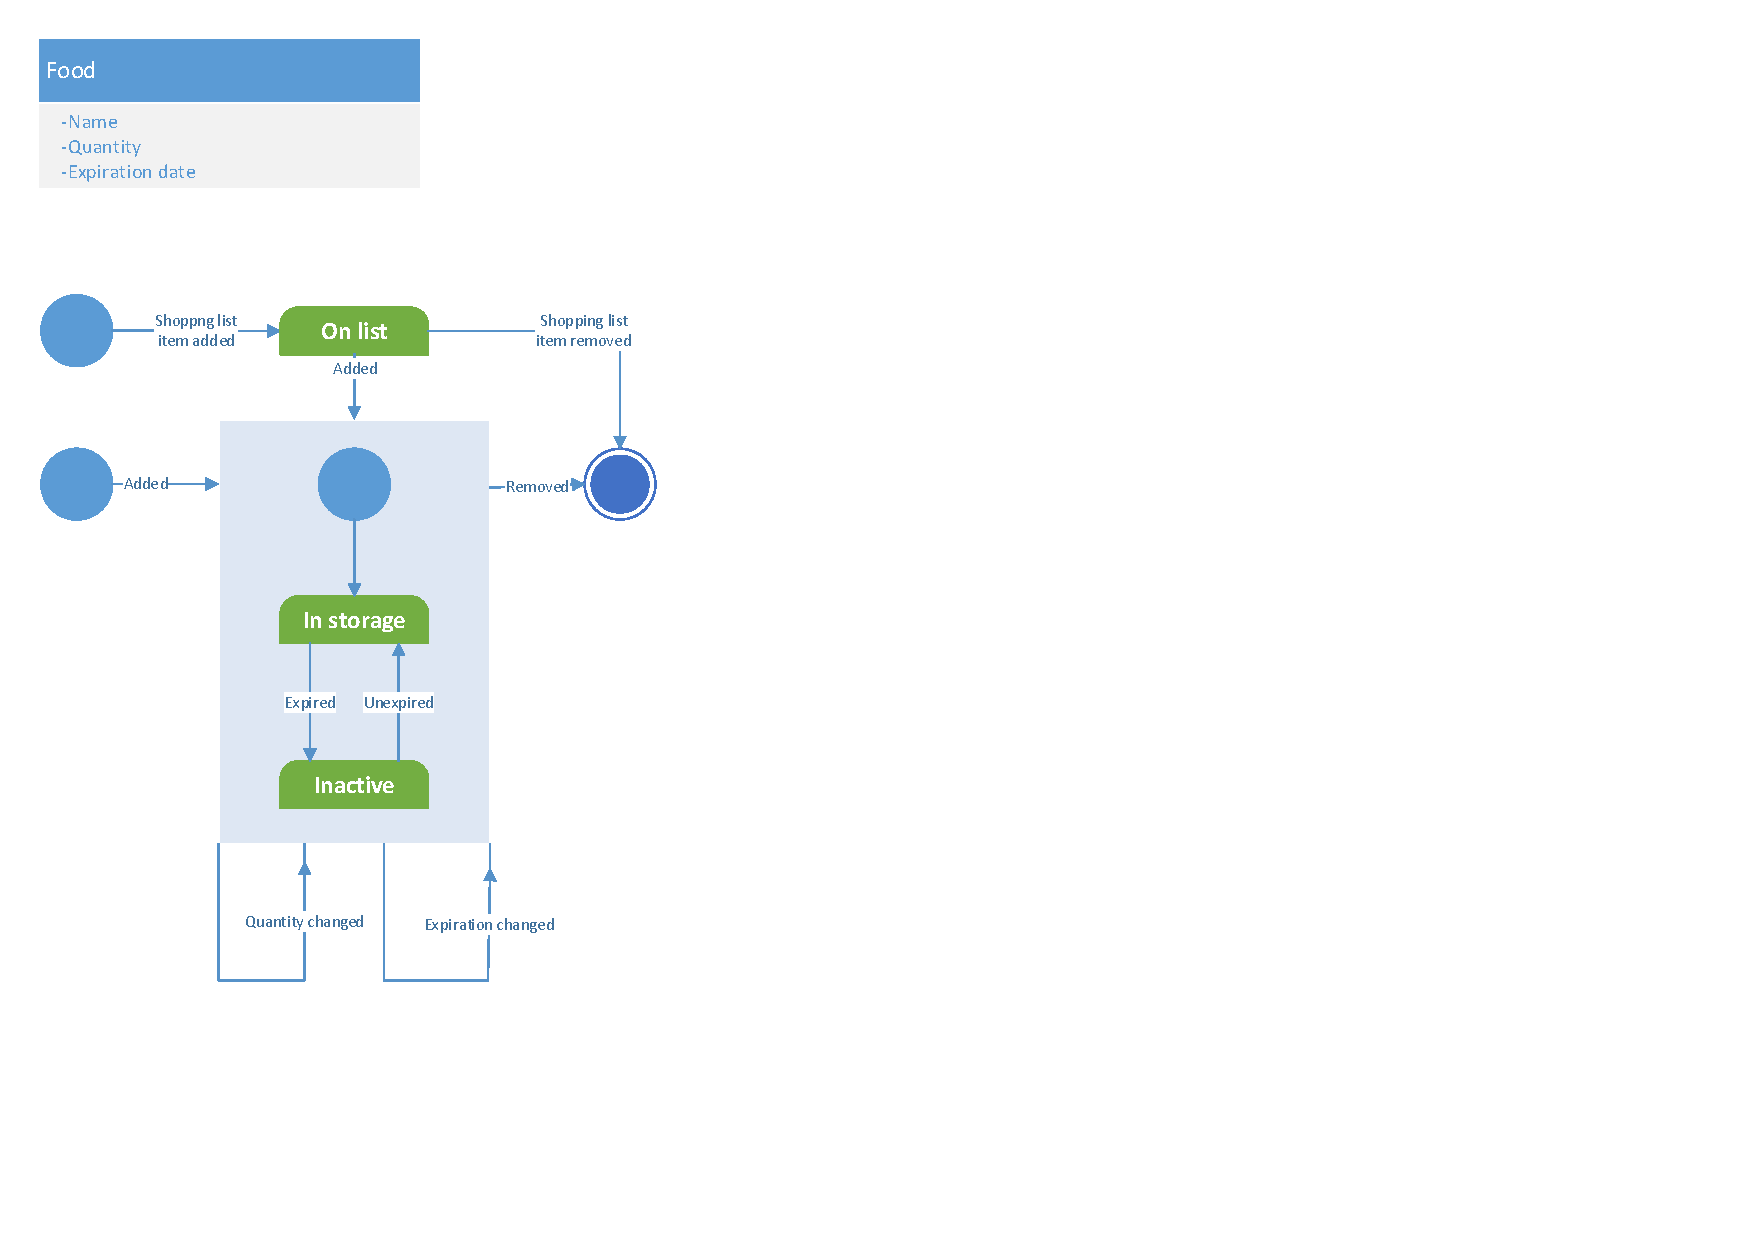
\includegraphics[clip=true, trim=0.5cm 4cm 18.5cm 0.5cm,  ]{Grafik/FoodPlanner/Food.pdf}
	\caption{Statemachine diagram for the Food class.} \label{FoodClass}
\end{figure}
An object of this class can be instantiated when the user either adds a shopping list item or adds a food item directly to their inventory. The two starting events for this class are therefore \textit{Shopping list item added} and \textit{Added}. The two start events sets the object's state to either \textit{On list} or \textit{In storage}. The On list state can be changed by the Add event, which sets the state to In storage, or by the \textit{Shopping list item removed} event, which terminates the object. The object can also have the state \textit{Inactive}, which can be set by the \textit{Expired} event and reset to the In storage state by the \textit{Unexpired} event. It is possible for an object in both the In storage and Inactive state to be effected by the \textit{Quantity changed} and \textit{Expiration changed} event, without changing the object's state. These two events can be iterated throughout an object's lifetime. The object can also be terminated from the In storage and Inactive state, by the \textit{Removed} event.   

\subsection{Meal Class}
Some of the event traces used to understand this class are:
\begin{itemize}
	\item \textit{Meal added} -> \textit{Change scale} -> \textit{Meal prepared}.
	\item \textit{Meal added} -> \textit{Change date} -> \textit{Meal prepared}.
	\item \textit{Meal added} -> \textit{Day passed} ->\textit{ Reschedule meal} -> \textit{Meal prepared}.
	\item \textit{Meal added} -> \textit{Change scale} -> \textit{Change date} -> \textit{Change scale} -> \textit{Meal prepared}.
\end{itemize}

An example of event traces that are not legal for this class are: \textit{Meal added} -> \textit{Day passed} -> \textit{Change Scale}.

\begin{figure}[H]
	\centering
	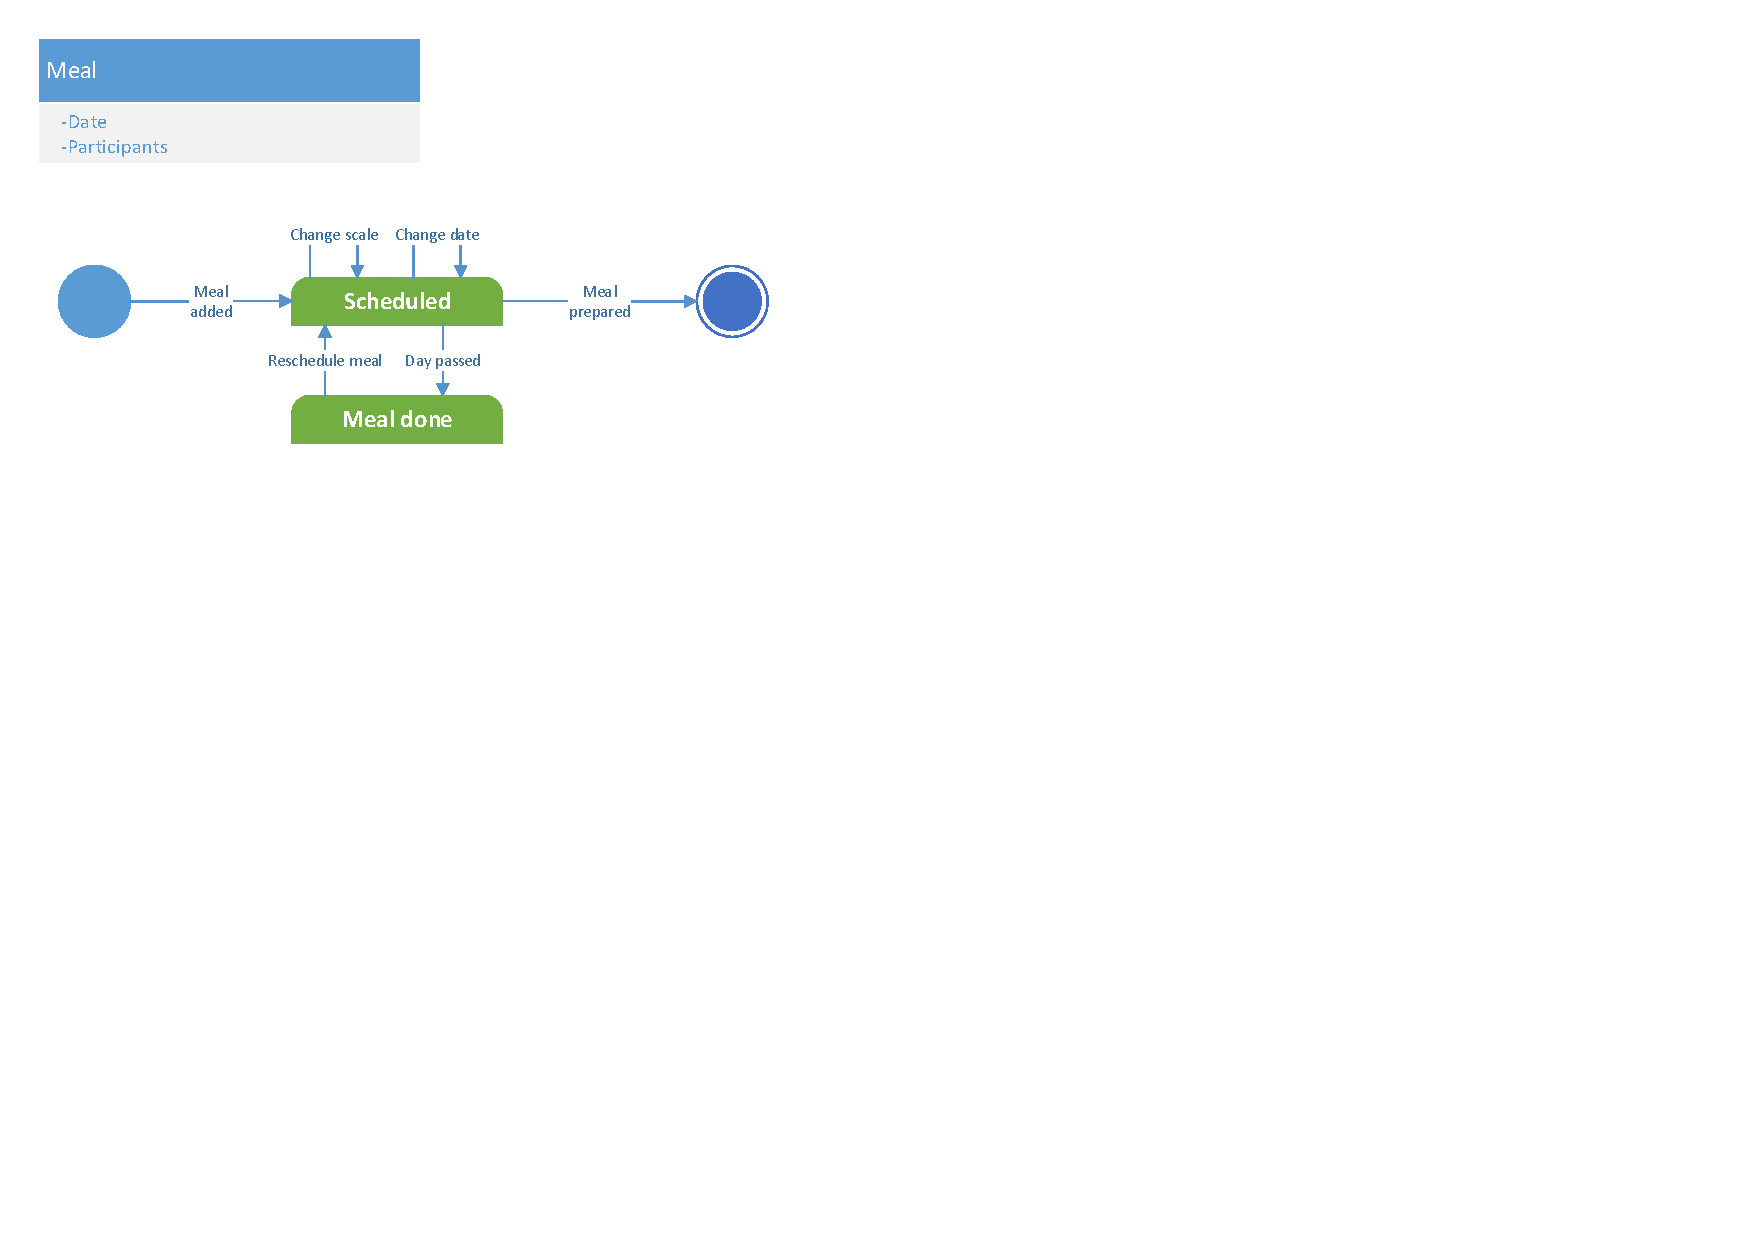
\includegraphics[clip=true, trim=0.5cm 13cm 16.5cm 0.5cm]{Grafik/FoodPlanner/Meal.pdf}
	\caption{Statemachine diagram for the Meal class.} \label{MealClass}
\end{figure}

An object of the meal class can be instantiated by the \textit{Meal added} event, and this sets the state of the object to \textit{Scheduled}. The events \textit{Change scale} and \textit{Change date} can be iterated throughout the object's lifetime, and does not change the state of the object. The object can also have the \textit{Meal done} state, which can be set by the \textit{Day passed} event and reset to the Scheduled state by the \textit{Reschedule meal} event. The object can only be terminated by the \textit{Meal prepared} event.

\subsection{User Class}
Some of the event traces used to better understand the events and flow of the User class are:

\begin{itemize}
	\item \textit{User registered} -> \textit{Preference added} -> \textit{Preference added} -> \textit{User deleted}.
	\item \textit{User registered} -> \textit{Preference added} -> \textit{Preference removed} -> \textit{User deleted}.
\end{itemize}

An event trace which is not legal for this class could be \textit{User registered} -> \textit{Preference removed} -> \textit{User deleted}.

\begin{figure}[H]
	\centering
	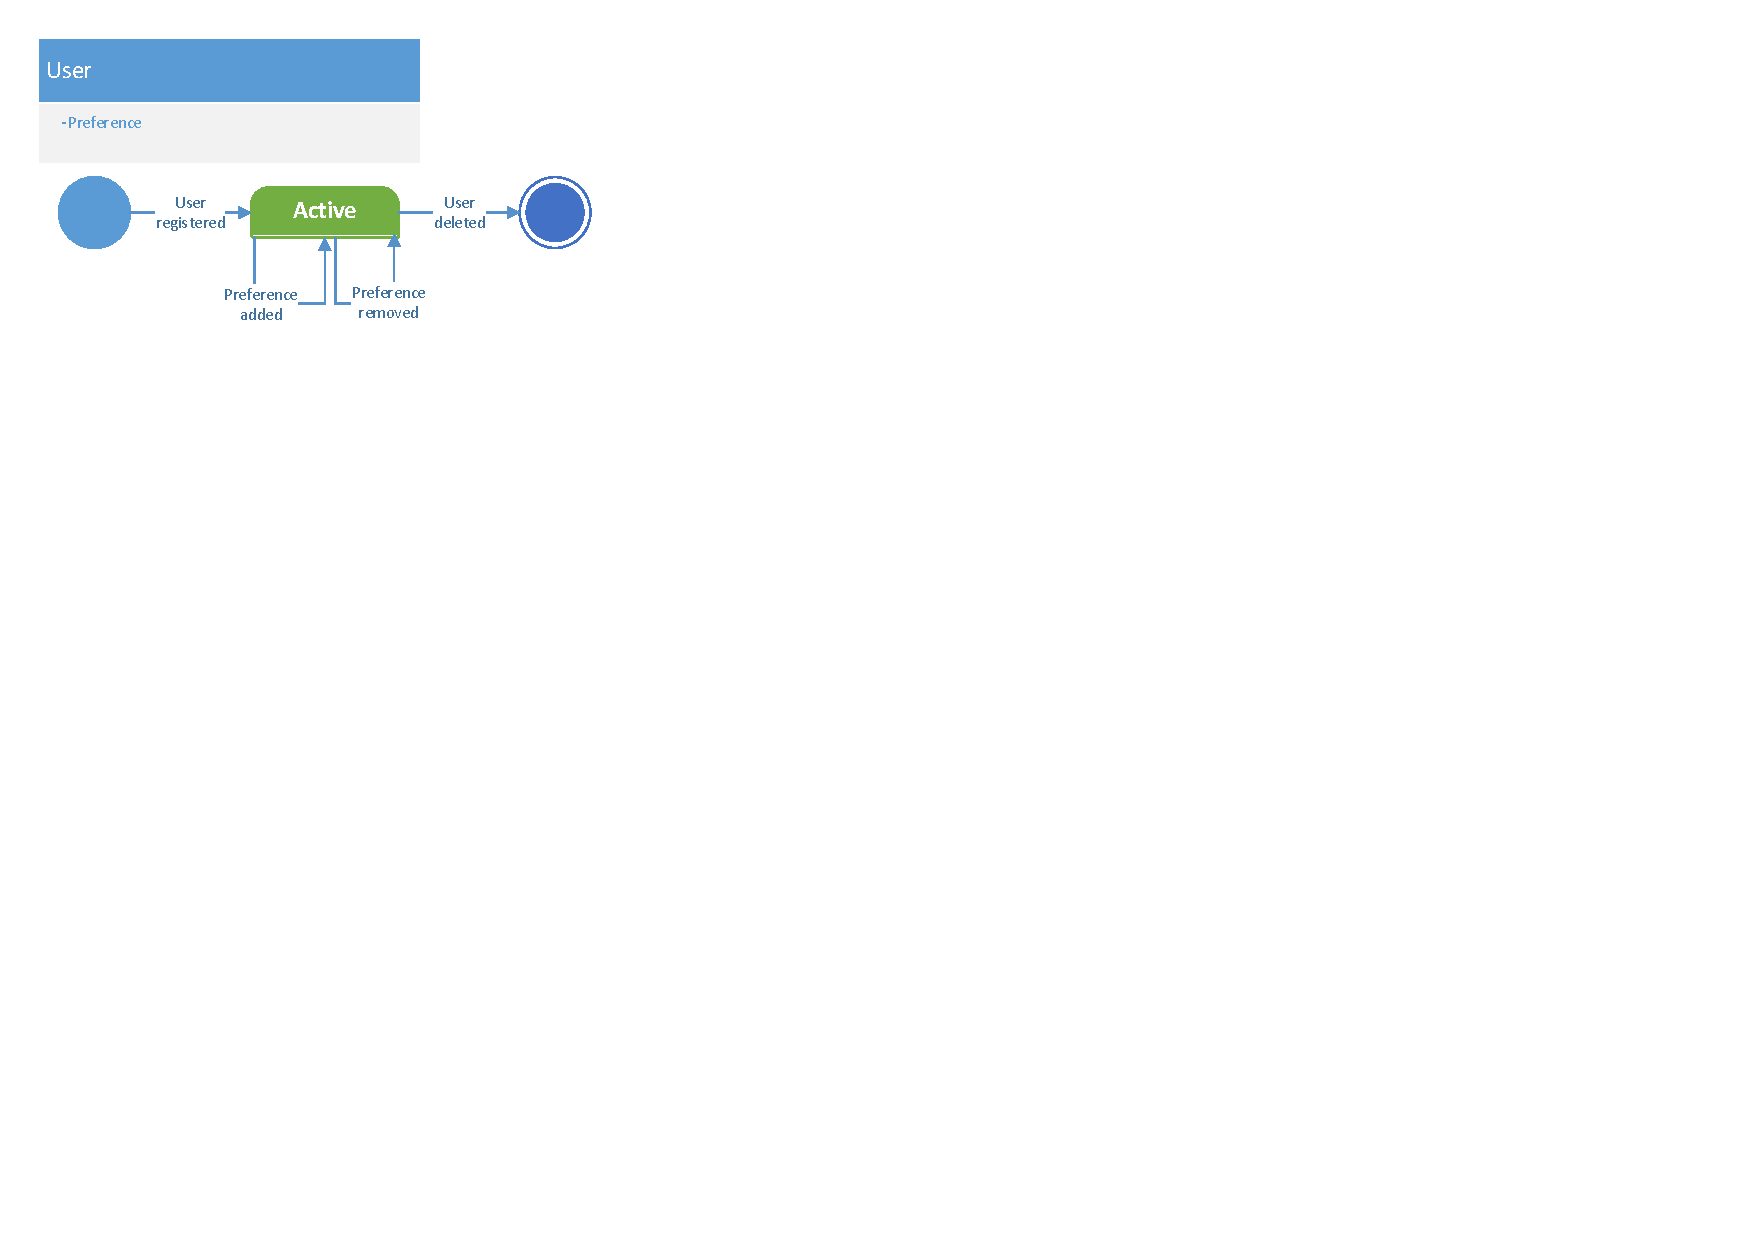
\includegraphics[clip=true, trim=0 14cm 5cm 0]{Grafik/FoodPlanner/UserSettings.pdf}
	\caption{Statemachine diagram for the User class.} \label{UserSettingsClass}
\end{figure}

This class can have an object instantiated by the \textit{User registration} event, and this event sets the object's state to \textit{Active}. From this state the \textit{Preference added} and \textit{Preference removed} event can be iterated throughout the object's lifetime. The object can only be terminated by the \textit{User deleted} event.


\subsection{Recipe Class}
Some of the event traces used to understand the Recipe class are:
\begin{itemize}
	\item \textit{Recipe added} -> \textit{Recipe removed}.
	\item \textit{Recipe added} -> \textit{Recipe found} -> \textit{Meal added} -> \textit{Meal removed}.
	\item \textit{Recipe added} -> \textit{Recipe found} -> \textit{Recipe found} -> \textit{Meal added} -> \textit{Meal removed}.
\end{itemize}

One of the event traces which are not legal for this class are:\textit{ Recipe added }-> \textit{Recipe found} - \textit{Meal removed}.

\begin{figure}[H]
	\centering
	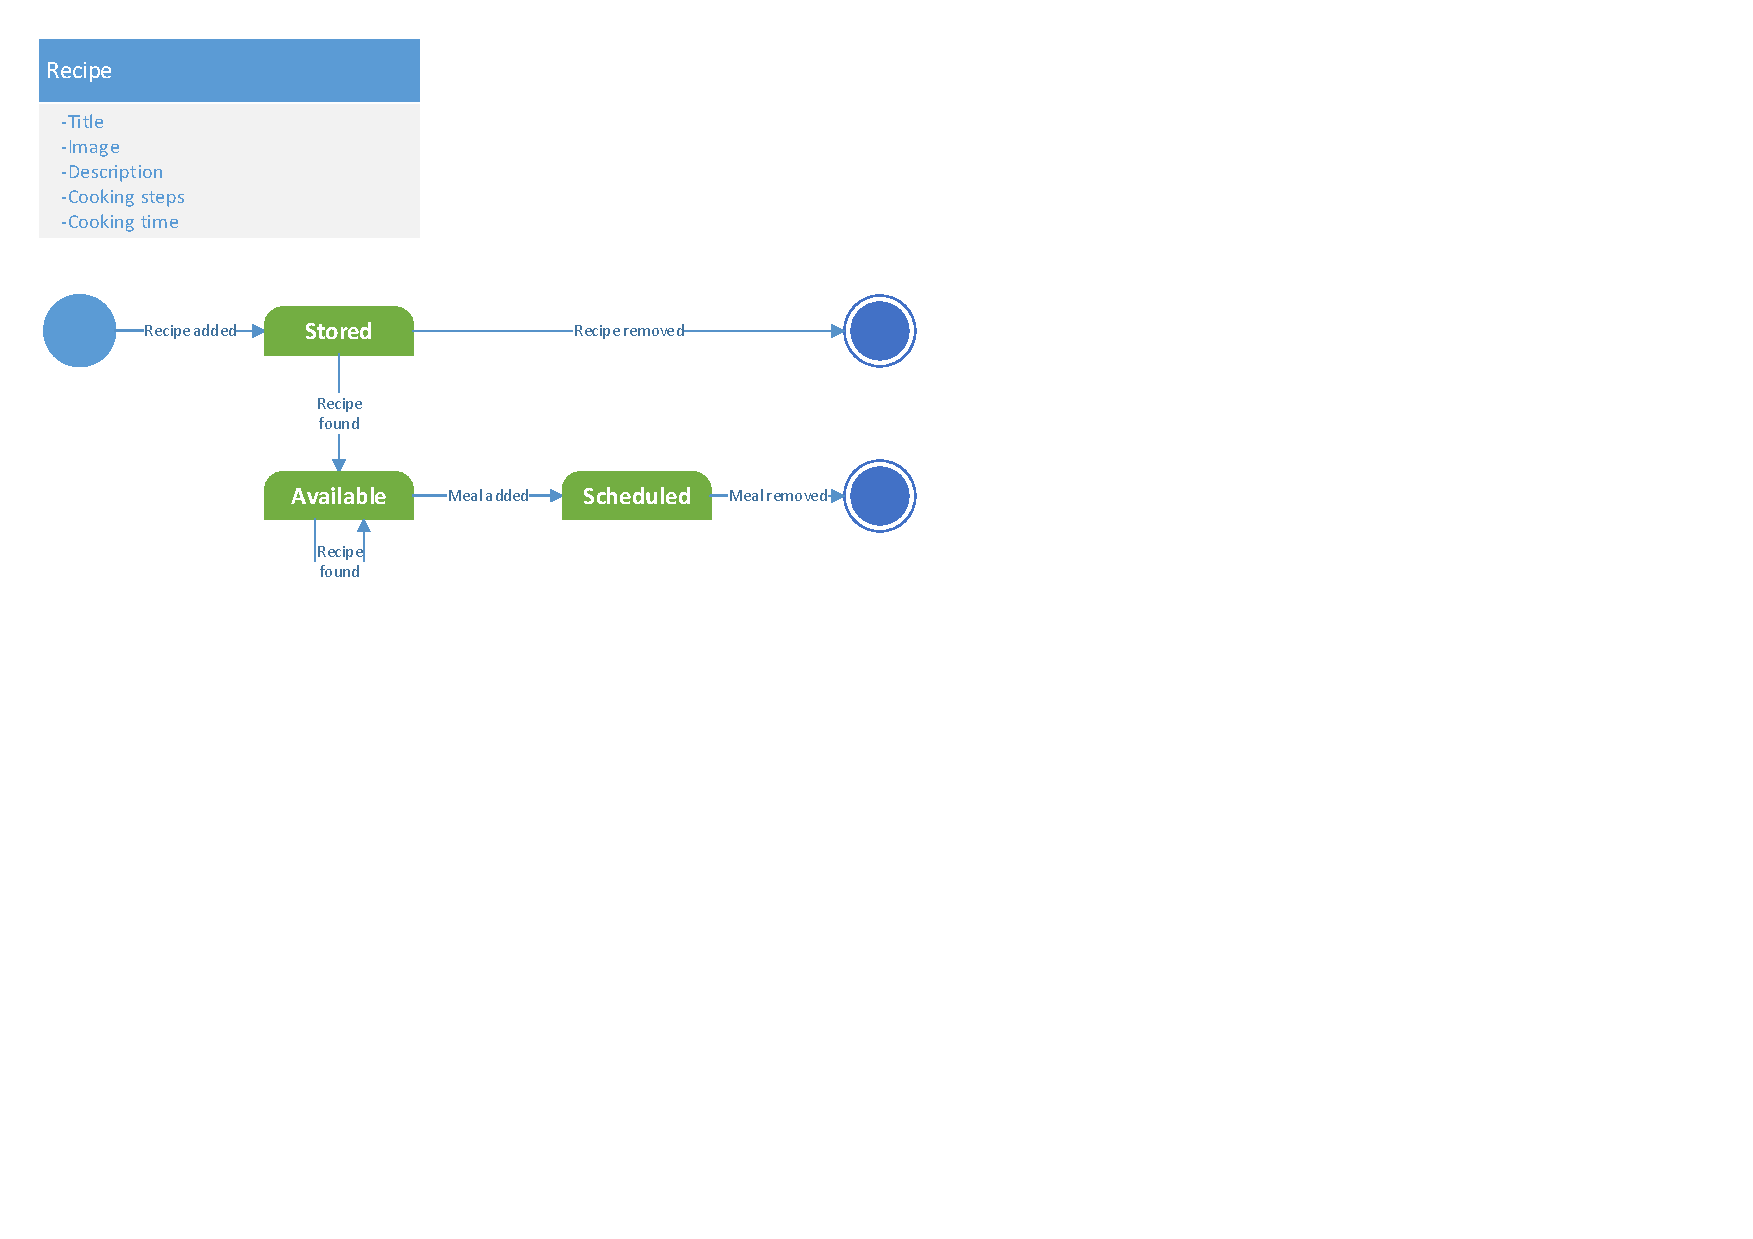
\includegraphics[clip=true, trim=0.5cm 11cm 14cm 0.5cm]{Grafik/FoodPlanner/Recipe.pdf}
	\caption{Statemachine diagram for the Recipe class.} \label{RecipeClass}
\end{figure}

An object of the Recipe class can only be instantiated by the \textit{Recipe added} event, and this event sets the state of the object to \textit{Stored}. From this state the \textit{Recipe removed} event can terminate the object. The \textit{Recipe found} event can change the object's state from Stored to \textit{Available}. The same event can also be iterated in this state, without changing the state. The \textit{Meal added} event can change the object's state to \textit{Scheduled}. From this state the \textit{Meal removed} event can terminate the object.

	\part{Application Domain}
		Anvendelsesområdet se side 296

\section{Usage}\label{Usage}
This section will describe the systems interaction with its surroundings. This will be done by making an actor specification and then presenting user pattern diagrams, which will be showcased in state machine diagrams.

\subsection{Actor specification}
\label{Actor_specification}
This system only contains one actor, which is the user of the system. The actor will be described by an actor specification.

\textbf{Objective:} A person who prepares meals, either for himself or for a household. The user's primary need is to plan his week in order to efficiently shop groceries and reduce food waste.

\textbf{Characteristic:} The system includes a user base of which the users have different needs and preferences.

\textbf{Example one:} User A is allergic to nuts and has to make meals which excludes these. When he is shopping he needs to look at the package info to make sure that the product does not contain traces of nuts.

\textbf{Example two:} User B is a young student who is in a relationship. He has a tight budget and a short time frame to shop in. The couple finds it difficult to sustain an overview of their shared storage of food. Therefore User B will sometimes buy products the couple do not need, for example, he might purchase milk even though they already have three litres stored. This will sometimes result in them not being able to use all the milk before it expires, which is bad for their shared budget and food waste.



\subsection{Use Cases}
The use cases shows how the actor interacts with the system to complete tasks. These interactions are shown in state machine diagrams. The diagrams show how the dynamic states can shift through interactions with the actor. Even though many of the details is excluded, it still gives an overview of the logic and flow behind the use cases.

The purpose of the diagram is to create an overview of the application domain's interactions with the system. This will be used to find requirements for the functions and user interface. There are three user pattern diagrams, each representing different areas of the system. The three diagrams showcase the user patterns in the:

\begin{itemize}
\item{Shopping list}
\item{Meal plan}
\item{Inventory}
\end{itemize}

When the user navigates the system, the user will undertake one of two roles. An administrative or a planning oriented role.
The option to go back or cancel have not been included in any of the diagrams, as their only contribution is to make the diagrams less readable and add redundant repetitions.

\Cref{Foodplan_Figure} shows the state machine diagram for planning meals. In this part of the system the user operates under the role of planning.

\begin{figure}[H]
	\centering
	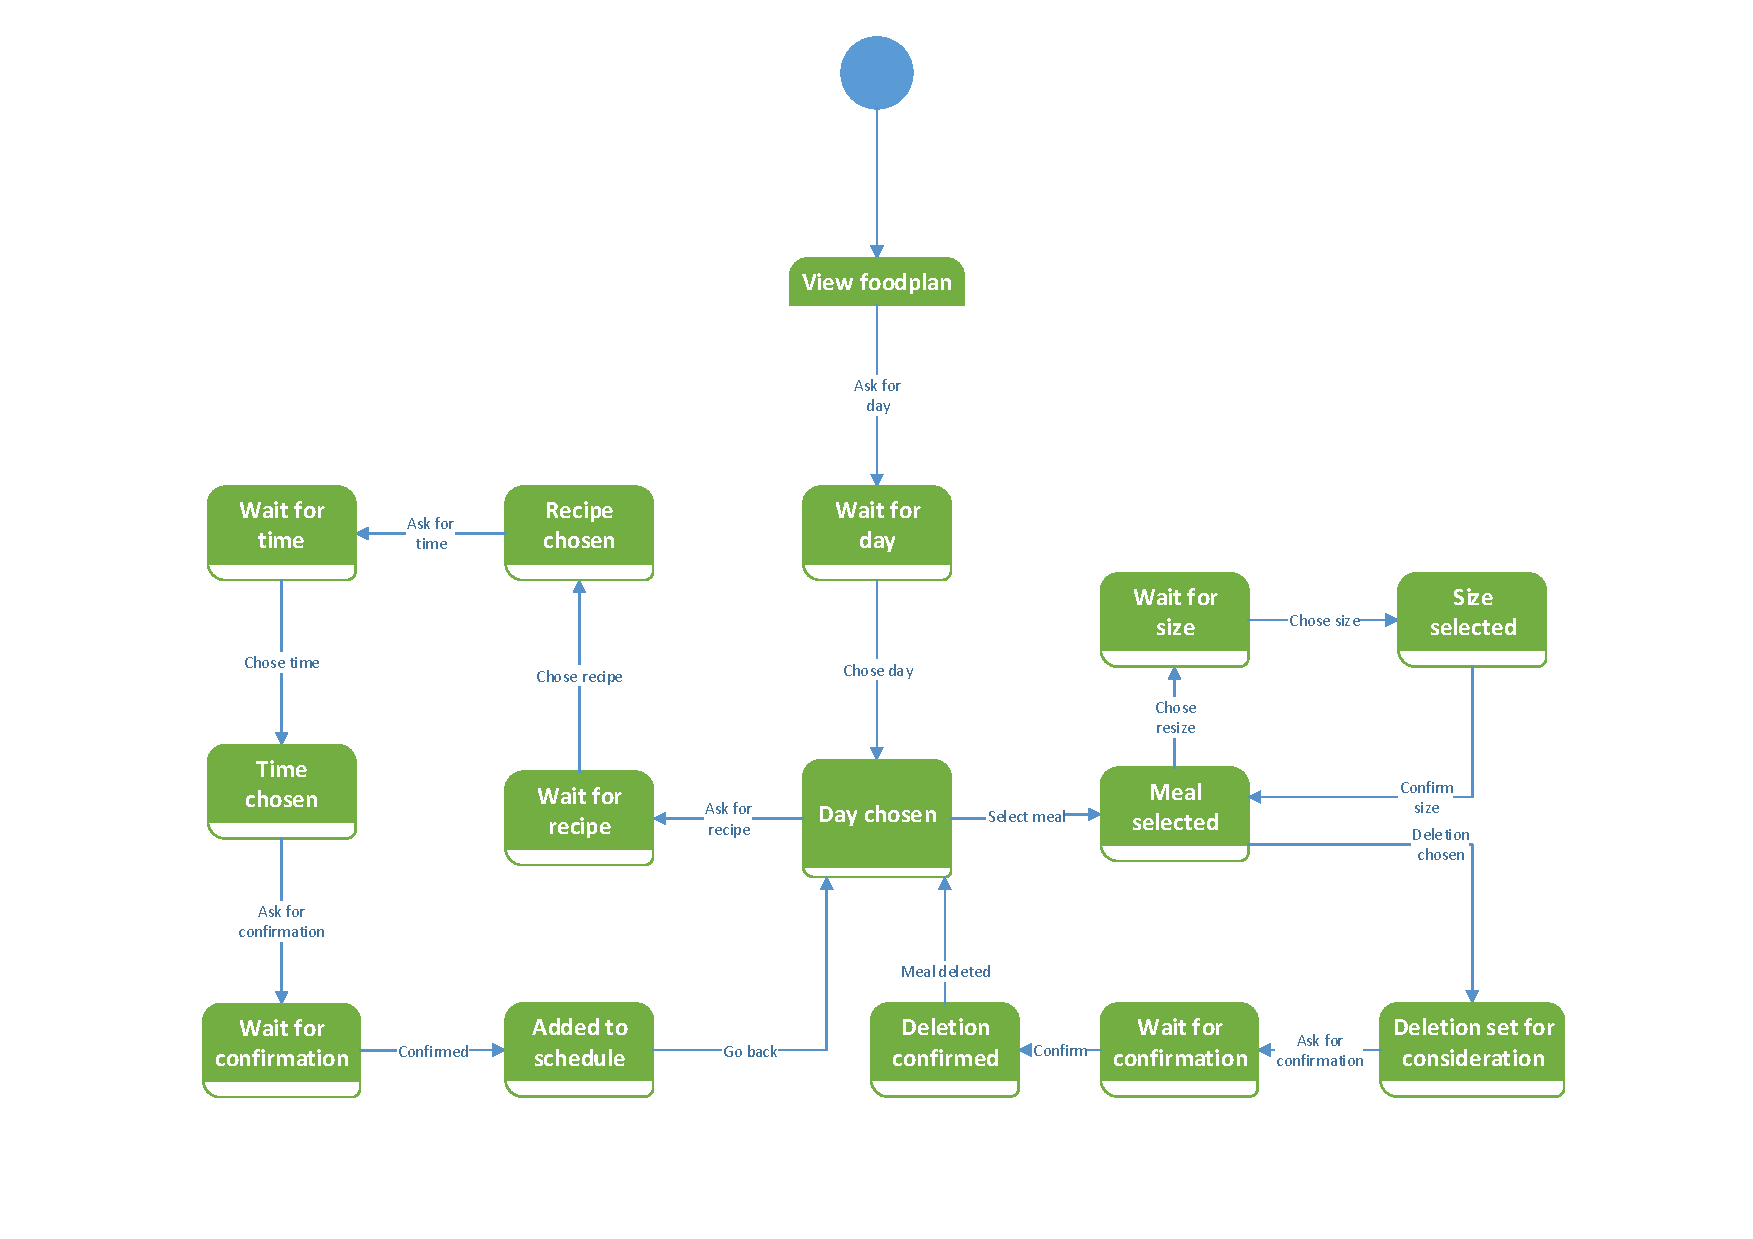
\includegraphics[width=1.0\textwidth]{ApplicationDomain/spViewFoodPlan.pdf} 
	\caption{State machine diagram for meal planning.}
	\label{Foodplan_Figure}
\end{figure}
When the user navigates to the meal plan part of the system, he will have to choose a day to view the meal plan for. From there the user can add a new meal to the plan or select an existing planned meal. If the user chooses to add a new meal, the system will ask for a recipe. The recipes the user can choose from varies depending on the user's preferences. If the user has chosen to avoid some products, recipes that contain those products will be excluded. When a recipe has been chosen, a time can be entered for when the meal should be prepared. After confirmation the meal will be added to the schedule.

The next two diagrams, \cref{Inventory_Figure} and \cref{spEditInventory}, are for the inventory. In this part of the system the user operates as an administrator.

\begin{figure}[H]
	\centering
	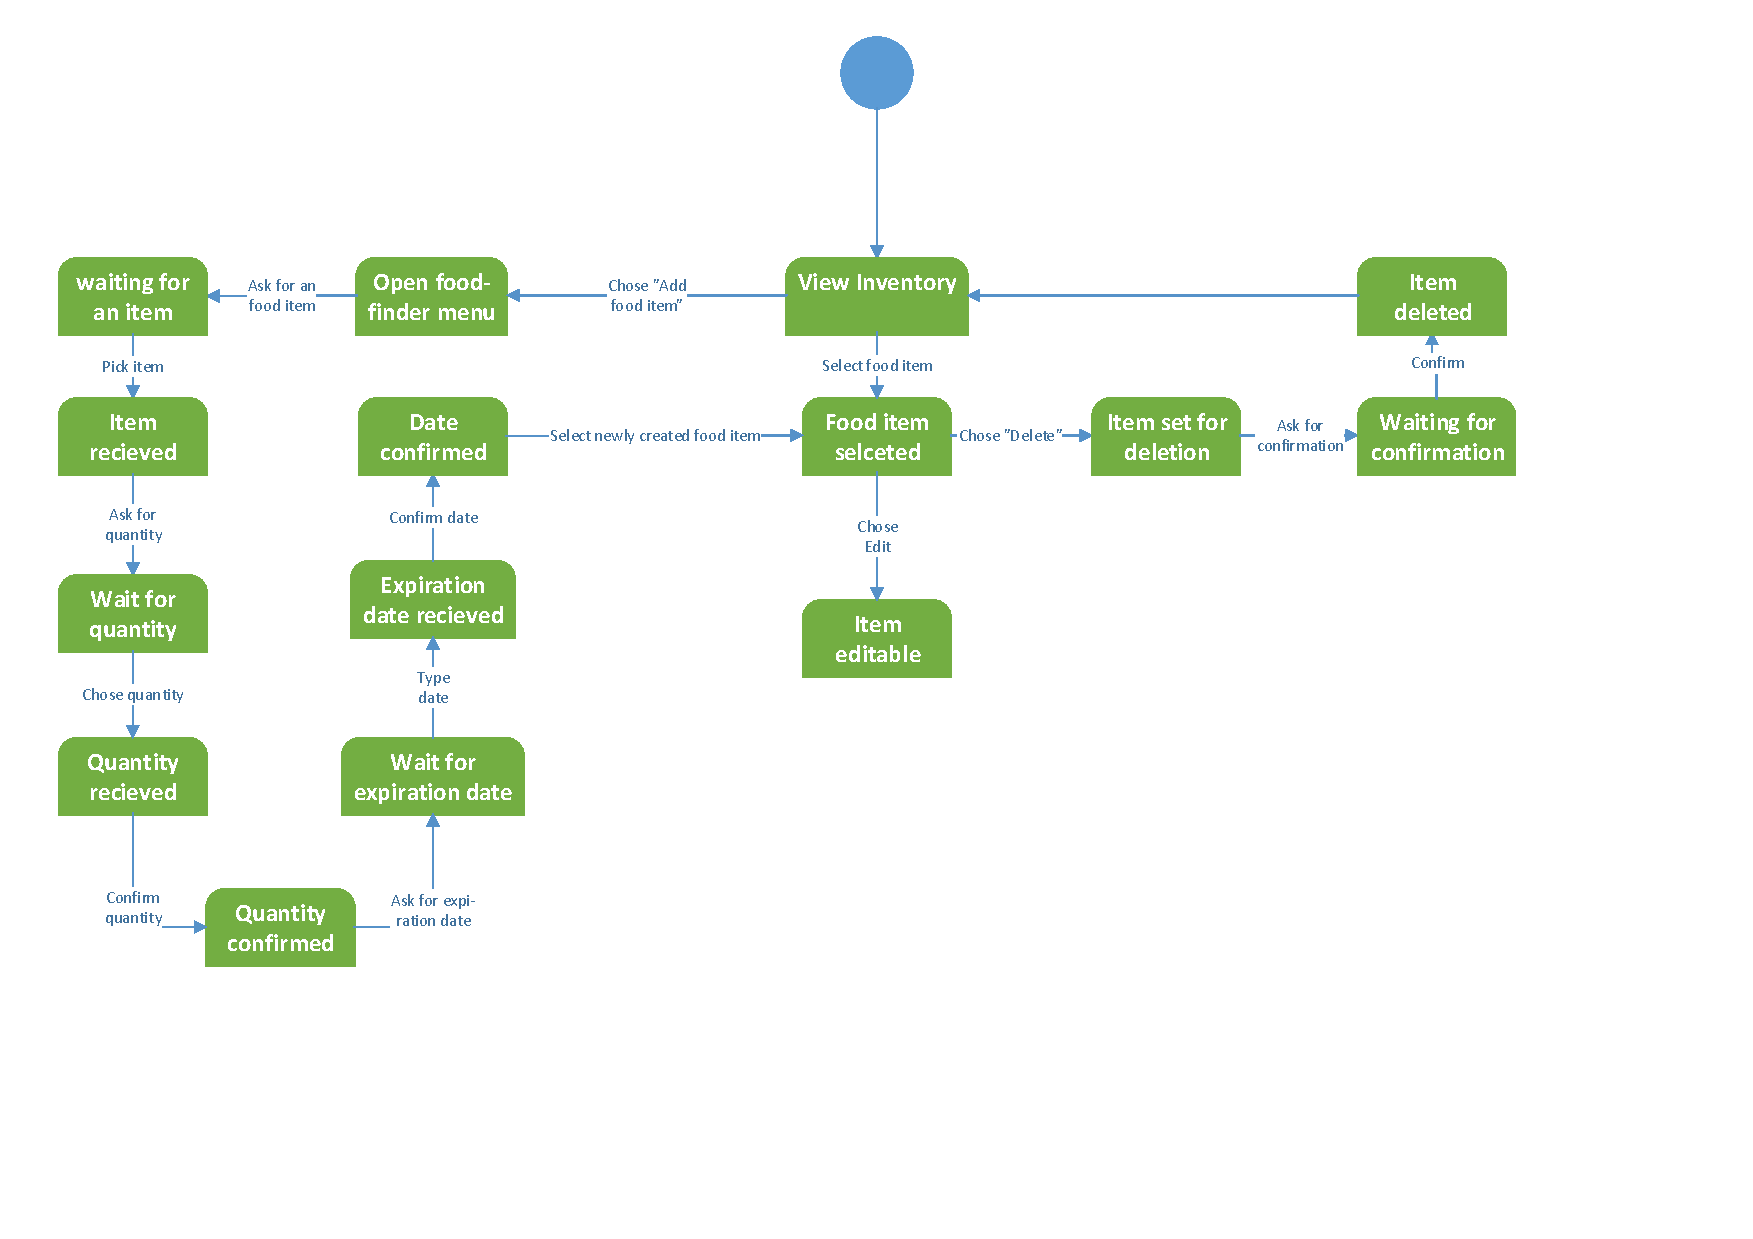
\includegraphics[width=1.0\textwidth, trim= 0 4cm 3cm 0]{ApplicationDomain/spViewInventory.pdf} 
	\caption{The \textit{View Inventory} state diagram}
	\label{Inventory_Figure}
\end{figure}
The user starts on the \textit{View Inventory} state where the inventory is shown. From here the user can choose from three different options: One that adds food to the inventory, another which allows the user to delete existing food items and a last option for editing food items. The edit option has its own diagram (see \cref{spEditInventory}). If the user chooses to add food, they will have to select food from a list. After a food item have been chosen, the system will ask for the user to select a quantity in order to know how much of the food item the user have acquired. For example, the user can buy five bananas or two hundred grams of flour. The user will afterwards have to enter when the food expires. When this is done the food will be added to the inventory. This leaves the user at the food item they have added, as if it was selected on the inventory screen. This is the same result as if the user chose to select a food item from the beginning. From here the user will be able to edit or delete a food item. \label{InvDesc}

When the user chooses to delete a selected item, the system will ask for a confirmation before it is deleted. If the user confirms, the system will delete the food item and go back to the view inventory state.


\Cref{spEditInventory}, is the last diagram which also covers the inventory. In this part of the system the user operates as an administrator.

\begin{figure}[H]
	\centering
	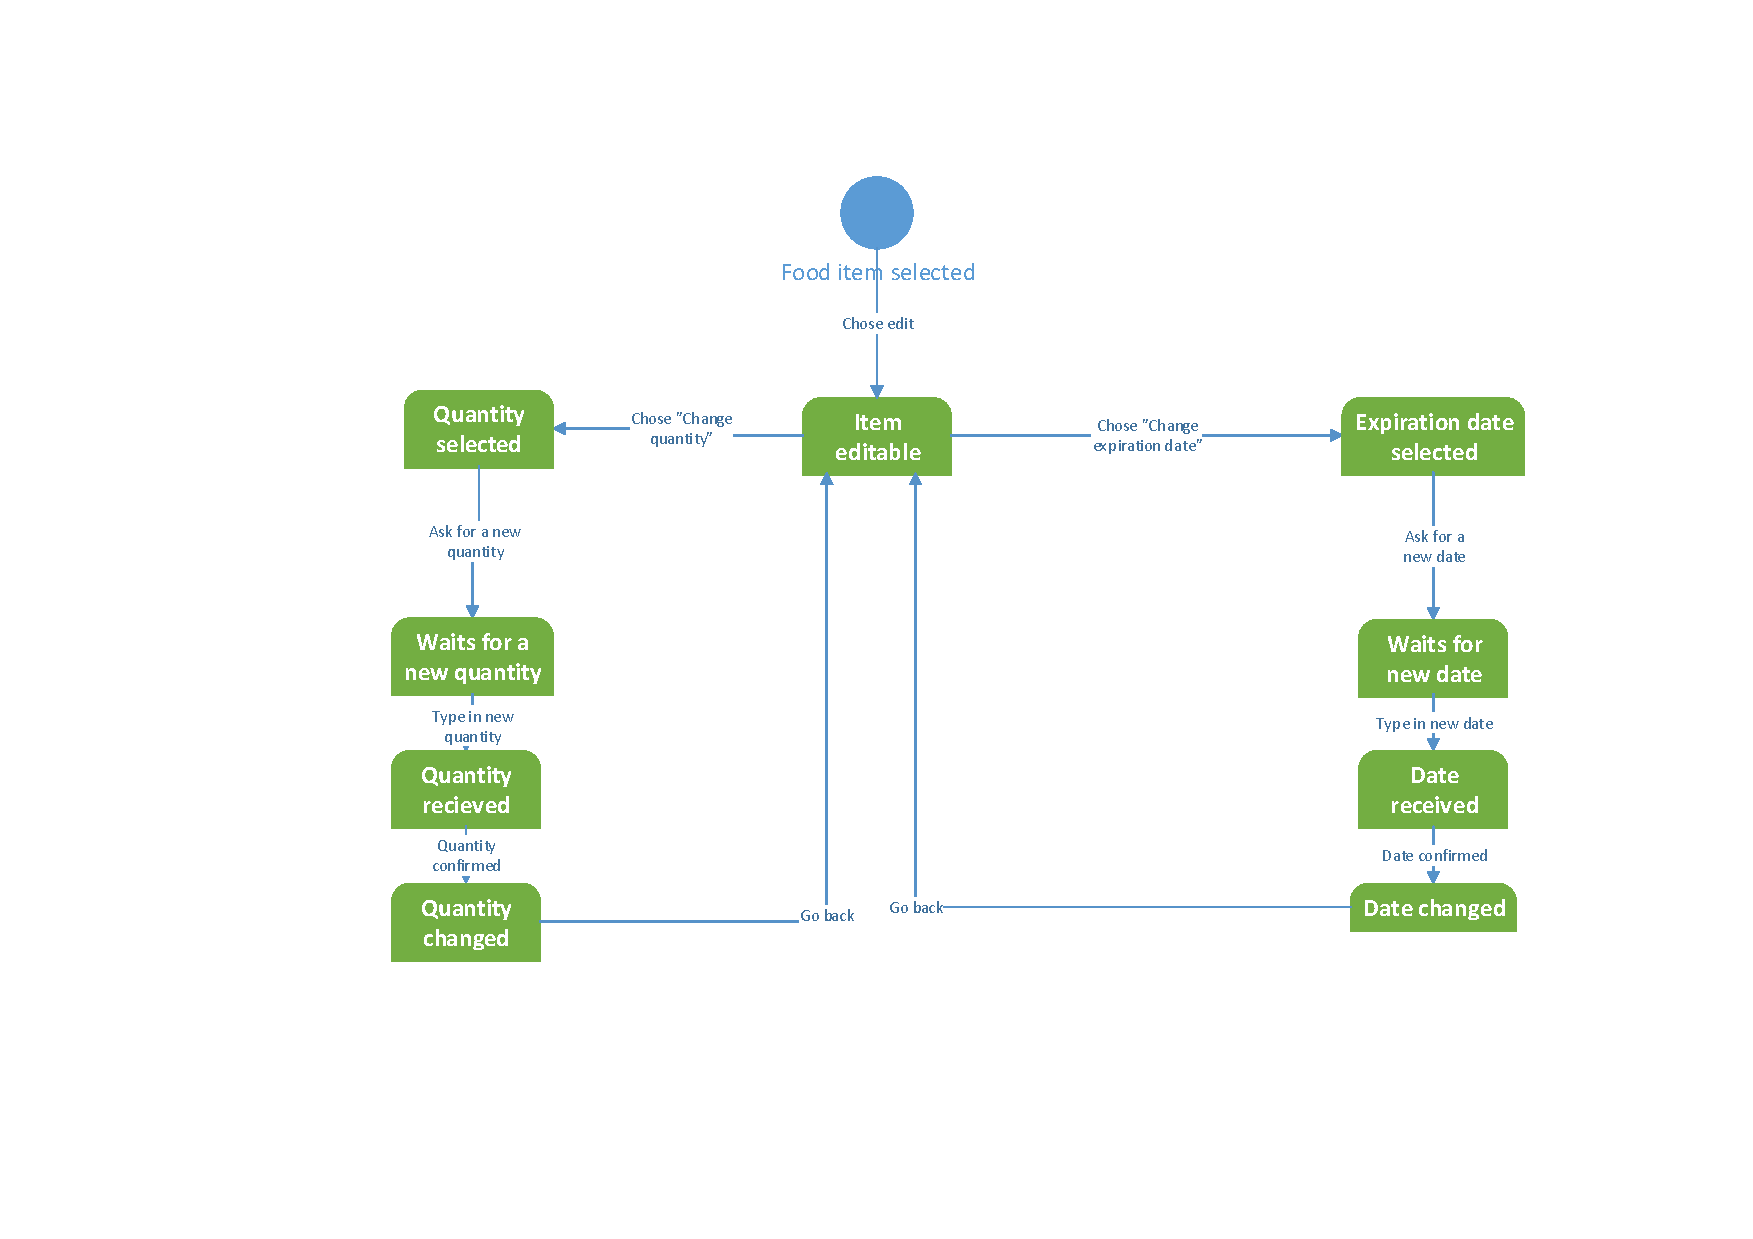
\includegraphics[width=1.0\textwidth, trim= 0 5cm 0 4cm]{ApplicationDomain/spEditInventory.pdf} 
	\caption{The \textit{Edit Inventory} state diagram.}
	\label{spEditInventory}
\end{figure}
The possible options in form of editing, is to change the quantity or expiration date. 
When choosing \textit{Change quantity} it works like the \textit{Change quantity} in the shopping list, which means that choosing an amount that leaves it at zero deletes the item, and leaving it below zero is not allowed. When the user tries to change the expiration date, the system prompts for a new date. All dates will be valid, which means that an item which was expired can go \textit{unexpired} as described at the diagram \cref{MealClass}. This also works the other way around as a fresh item can expire if the date changes to the day prior to the day it expires.

\subsection*{Summary}
The actor specification and use cases helped to establish an understanding of how the user base will interact with the system. By defining the use cases, some flaws in the design were discovered which resulted in varies corrections.
%Funktioner - beskrivelse af systemets funktionalitet se kap 7
%	Komplet funktionsliste
%	Specifikation af funktioner
	
	\chapter{Functions}
	\section{Function definitions}
	The diagrams in \ref{Usage} contain different functions these functions have been given a name and listed in the following tables, where they have been assigned a complexity of Simple, Medium or Complex, and they have been assigned one or more of the following types; Read, Update, Calculate or Signaling. The more complex functions are further elaborated under each table.
\begin{table}[H]
	\centering
	\caption{Shopping list}
	\begin{tabular}{|l|l|l|}\hline
		\textbf{Function}&\textbf{Complexity}&\textbf{Type}\\\hline
	  Update shopping list  &  Complex & Update \\\hline
	  View shopping list    &  Simple  & Read   \\\hline
  \end{tabular}
  \begin{flushleft}
    \textbf{Update shopping list:} The update function will be triggered by the signal function from the inventory "Update shopping list" function". When a meal is added or removed from the food plan. The shopping list should represent what ingredients that is needed to prepare the meals in the foodplan.
  \end{flushleft}
	\caption{Food plan:}
  \begin{tabular}{|l|l|l|}\hline
		\textbf{Function}&\textbf{Complexity}&\textbf{Type}\\\hline
	  Add meal              &  Complex & Calculate, update \\\hline
	  Remove meal           &  Simple  & Update            \\\hline
	  View food plan        &  Simple  & Read              \\\hline
  \end{tabular}
  \begin{flushleft}
    \textbf{Add meal:} The add meal function is given the complex status as it involves many actions in order to add the meal onto the schedule. When the user goes trough the steps necessary to schedule a meal, the system will do a lookup in order to create a list of needed ingredients. This list will be compared with what the user has in the inventory, and any ingredients that is not present on the list will then be added to the shopping list. This is were the previously described function comes into play.
  \end{flushleft}
	\caption{Inventory:}
  \begin{tabular}{|l|l|l|}\hline
		\textbf{Function}&\textbf{Complexity}&\textbf{Type}\\\hline
	  View inventory        &  Simple  & Read   \\\hline
	  Update shopping list  &  simple  & Signal \\\hline
	  Add Item              &  Complex & Update \\\hline
	  Edit Item             &  Complex & Update \\\hline
	  Remove Item           &  Simple  & Update \\\hline
  \end{tabular}
  \begin{flushleft}  	  
    \textbf{Add item:} The add item function have been marked as complex. The function is complex as there many steps involved when adding an item, see \Cref{InvDesc} for a description of these steps. By having this function the user is able to add food to their storage manually.
    
    \textbf{Edit item:} The edit item function is complex as well. If the user changes the expiration date on an item,it could potential update the inventory as an item can "unexpire". The same goes for changing the quantity of an food item. If the quantity reaches zero the item will be deleted, and therefore an update in the storage will be needed.
  \end{flushleft}
\end{table}
\input{ApplicationDomain/UserinterFace}
Den tekniske platform?

    \part{Summary}

    \part{Annexes}
    
    \printbibliography
    
    % list of fxnotes that needs to be fixed
    \listoffixmes

\end{document}